\begin{figure}[!htbp]
  \centering
  \begin{tabular}{m{15cm}}
  \toprule
  \begin{center}
  
\includegraphics[width=0.55\linewidth]{figures/case/case1.png}
  \end{center}\\
  {\footnotesize\textbf{Instruction:} Convert it to a table.}\\
  {\footnotesize\textbf{\mimovlrl{}:}} \\
  \begin{center}
  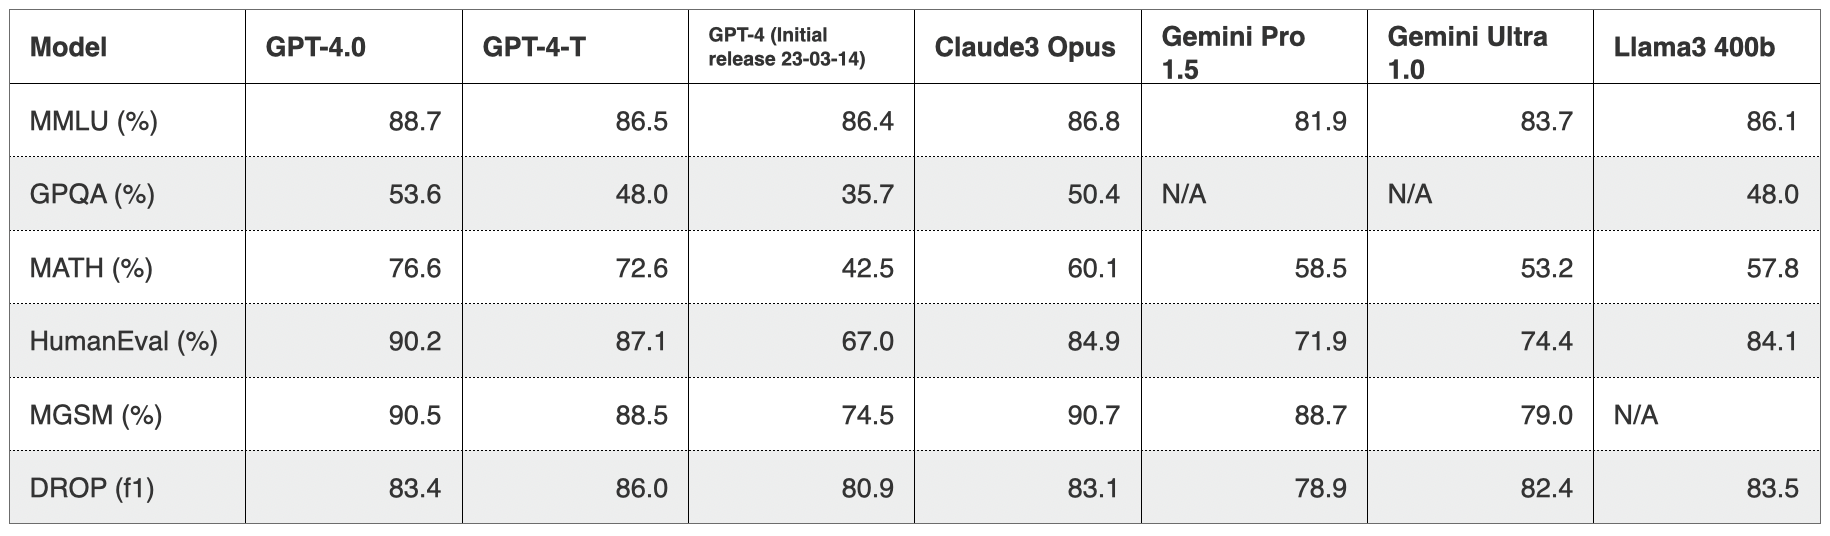
\includegraphics[width=0.75\linewidth]{figures/case/case1-2.png}
  \end{center} \\
  
  \midrule
  
  \begin{center}
  
\includegraphics[width=0.55\linewidth]{figures/case/case2.png}
  \end{center} \\
  {\footnotesize\textbf{Instruction:} Answer the question in image.} \\
  {\footnotesize \textbf{\mimovlrl{}:} \texttt{<think>...</think>} To solve for the tension in the wire, we use the \textbf{equilibrium of torques} about the hinge point $ P $. For a beam in equilibrium, the sum of clockwise torques equals the sum of counterclockwise torques.  

\textbf{Step 1: Identify Forces and Torques}

\quad - Beam’s weight ($ 425 \, \text{N} $): Acts downward at the beam’s midpoint (since it is uniform). The beam’s length is $ 8.4 \, \text{m} $, so the midpoint is $ \frac{8.4}{2} = 4.2 \, \text{m} $ from $ P $.  

\quad - Block’s weight ($ 720 \, \text{N} $): Acts downward at $ 8.4 \, \text{m} $ from $ P $. 

\quad - Tension in the wire ($ T $): Acts at $ 3.4 \, \text{m} $ from $ P $ at an angle of $ 23^\circ $ above the horizontal. Only the \textbf{vertical component} of tension ($ T \sin 23^\circ $) contributes to torque (the horizontal component acts along the beam, so its torque about $ P $ is zero).  


\textbf{Step 2: Calculate Torques}

Torque is defined as $ \text{force} \times \text{perpendicular distance from pivot} $.  

\quad - Clockwise torques (from the beam and block weights):  
  - Beam’s weight: $ 425 \, \text{N} \times 4.2 \, \text{m} = 1785 \, \text{N·m} $  
  - Block’s weight: $ 720 \, \text{N} \times 8.4 \, \text{m} = 6048 \, \text{N·m} $  
  - Total clockwise torque: $ 1785 + 6048 = 7833 \, \text{N·m} $  

\quad - Counterclockwise torque (from tension’s vertical component):  
  - Tension’s vertical component: $ T \sin 23^\circ $  
  - Perpendicular distance from $ P $ to the wire: $ 3.4 \, \text{m} $  
  - Torque from tension: $ T \sin 23^\circ \times 3.4 \, \text{m} $  


\textbf{Step 3: Solve for Tension} 

In equilibrium, clockwise torque = counterclockwise torque:  
$
T \sin 23^\circ \times 3.4 = 7833
$  

Solve for $ T $:  
$
T = \frac{7833}{3.4 \times \sin 23^\circ}
$  

Using $ \sin 23^\circ \approx 0.3907 $:  
$
T = \frac{7833}{3.4 \times 0.3907} \approx \frac{7833}{1.328} \approx 5900 \, \text{N}
$  


\textbf{Final Answer}  
The tension in the wire is approximately $ \boldsymbol{5900 \, \text{N}} $.
}\\
  \bottomrule
  \end{tabular}\\
\caption{Examples of \mimovl{} solving complicated problems.}
\label{fig:case_main}
\end{figure}
